\section{\color{blue}{Model Conversion from SAPHIRE to OpenPSA}}

% %----------------------------------------
% Section: Probabilistic Risk Assessment Model Structure
%----------------------------------------

\subsection{\color{yellow}{Probabilistic Risk Assessment Model Structure}}
\label{sec:pra_model_structure}

Probabilistic Risk Assessment (PRA) model generation is a crucial step in the design, operation, and decommissioning phases of a nuclear power plant (NPP). Different PRA software tools implement distinct methods for model generation, storage, and exchange. Understanding these methods is essential for enhancing interoperability and advancing tool capabilities. In this work, we focus on two representative tools: SAPHIRE (via its SAPHSOLVE solver) and SCRAM (via the Open‑PSA Model Exchange Format).

\subsubsection{\color{yellow}{SAPHSOLVE Models}}
\label{sec:saphsolve_models}

SAPHIRE’s quantification engine, SAPHSOLVE, exposes two primary solvers—Fault Tree Solver and Event Tree/Sequence Solver—via a JSON‑based remote interface. Below we outline SAPHIRE’s background and the structure of its input/output files.

\paragraph{Overview of SAPHIRE}
SAPHIRE is a comprehensive software package for PRA, documented in a seven‑volume manual \cite{24}:
\begin{enumerate}
  \item \textbf{Volume 1:} Overview of capabilities and summary of subsequent volumes.
  \item \textbf{Volume 2:} Technical reference covering fault‑tree logic, minimal cut‑sets, probability concepts, importance measures, uncertainty, and seismic calculations.
  \item \textbf{Volume 3:} User guide describing each feature in detail.
  \item \textbf{Volume 4:} Tutorial on building a PRA database using a simple example.
  \item \textbf{Volume 5:} Guide to SAPHIRE’s workspace types.
  \item \textbf{Volume 6:} Quality assurance methods, testing, and configuration control.
  \item \textbf{Volume 7:} Data loading, conversion methods, and validation.
\end{enumerate}
Users interact via a graphical user interface (GUI) or an Application Programming Interface (API) that orchestrates nine specialized engines:
\begin{itemize}
  \item \emph{Fault Tree Solver}: Generates cut‑sets from fault‑tree logic and basic event data.
  \item \emph{Event Tree/Sequence Solver}: Computes end‑states and associated cut‑sets for event trees.
  \item \emph{Cut Set Post‑Processor}: Applies rule files to update cut‑sets without regeneration.
  \item \emph{Cut Set Updater}: Ensures minimality of cut‑sets after post‑processing.
  \item \emph{Event Tree Linker}: Defines dependencies between fault‑tree and event‑tree constructs.
  \item \emph{Cut Set Partition Processor}: Partitions cut‑sets into end‑states.
  \item \emph{Change Set Processor}: Updates basic event data via change sets.
  \item \emph{Uncertainty Sampler}: Performs Monte Carlo and Latin Hypercube sampling.
  \item \emph{End‑State Gather}: Aggregates cut‑sets by end‑state.
\end{itemize}
For remote web‑based quantification, only the Fault Tree Solver and Event Tree/Sequence Solver are invoked via SAPHSOLVE.

\paragraph{SAPHSOLVE Model Structure}
SAPHSOLVE uses JavaScript Object Notation (JSON) \cite{37} for its input (``\texttt{.jsonp}’’) and output (``\texttt{.jsonc}’’) files. This format was chosen for its lightweight, self‑describing nature and ease of integration in web environments \cite{15}.

\paragraph{Input File Specification}
The input file (\texttt{.jsonp}) comprises:
\begin{itemize}
  \item \textbf{Header:} Model metadata and truncation parameters.
  \item \textbf{System Gate List:} Definitions of top‑level system gates.
  \item \textbf{Fault Tree List:} Logic expressions for each fault tree.
  \item \textbf{Sequence List:} Event‑tree definitions mapping fault‑tree outputs to sequences.
  \item \textbf{Event List:} Basic event failure rates and initiating event frequencies.
\end{itemize}
Each file represents either a single fault tree or a combined fault/event‑tree model. All models used in this study are available in the project repository \cite{38}.

\begin{figure}[htbp]
  \centering
  % \includegraphics[width=0.7\textwidth]{saphsolve_input_structure}
  \caption{General structure of the SAPHSOLVE input file \cite{15}.}
  \label{fig:saphsolve_input}
\end{figure}

\paragraph{Output File Specification}
The output file (\texttt{.jsonc}) returns:
\begin{itemize}
  \item \textbf{General Information:} Solver version, file path, and timestamp.
  \item \textbf{Truncation Parameters:} Values used during cut‑set generation.
  \item \textbf{Workspace Pair:} Phase (fault or event tree) and model identifier.
  \item \textbf{Sequence Results:} For each sequence or fault tree, the number of cut‑sets, total failure probability, and detailed cut‑set lists.
\end{itemize}

\begin{figure}[htbp]
  \centering
  % \includegraphics[width=0.7\textwidth]{saphsolve_output_structure}
  \caption{General structure of the SAPHSOLVE output file \cite{15}.}
  \label{fig:saphsolve_output}
\end{figure}

\subsubsection{\color{yellow}{Open‑PSA Model Exchange Framework}}
\label{sec:openpsa_mef}

The Open‑PSA \acrshort{mef} \cite{36} was developed to enable software‑independent PRA model sharing. It uses \acrshort{xml} for its explicit, hierarchical representation of model constructs.

\paragraph{Overview of SCRAM}
It operates via a command‑line interface, performing fault‑tree and event‑tree quantification, cut‑set generation, importance measures, and uncertainty analyses.

\paragraph{SCRAM Model Structure}
SCRAM adheres to a five‑layer XML architecture (Figure~\ref{fig:openpsa_arch}):
\begin{enumerate}
  \item \textbf{Stochastic Layer:} Probability distributions of basic event failure rates.
  \item \textbf{Fault Tree Layer:} Logical structure of fault trees.
  \item \textbf{Meta‑Logical Layer:} Common‑cause groups, delete terms, and recovery rules.
  \item \textbf{Event Tree Layer:} Initiating events and consequences.
  \item \textbf{Report Layer:} Computed results and importance measures.
\end{enumerate}

\begin{figure}[htbp]
  \centering
  % \includegraphics[width=0.7\textwidth]{openpsa_architecture}
  \caption{Architecture of the Open‑PSA Model Exchange Format \cite{36}.}
  \label{fig:openpsa_arch}
\end{figure}

Historically, the transfer of PRA models between tools has been full of challenges. Early efforts, such as the NRC's Models and Results Database (MAR-D), provided a centralized repository for PRA data, supporting the migration of models between mainframe and PC based tools (e.g., IRRAS, SARA, SETS, FRANTIC). While MAR-D enabled the exchange of event trees, fault trees, and associated data within the SAPHIRE ecosystem, it was not designed as a general purpose model exchange framework. Subsequent attempts to enable model exchange between tools such as CAFTA, RiskA, and RiskSpectrum have been limited in scope, often requiring significant manual intervention and lacking support for large or complex models. Notably, the import of SAPHIRE MAR-D files into CAFTA is restricted to logic files and is not scalable for large PRA models. Other efforts, such as the conversion of RiskSpectrum models to CAFTA or OpenPSA, have been either unsuccessful or undocumented.

The MEF framework that has been developed for this study operates at the quantification engine level, enabling the conversion of SAPHIRE models to the OpenPSA format. To illustrate the model conversion process, a simple PRA model is used, consisting of a single event tree linked to four fault trees. The event tree models the release of gas on an offshore platform, with subsequent functional events representing the gas detection system, two isolation valve subsystems (A and B), and a blowdown valve subsystem. The endpoints of the event tree branches correspond to different consequence scenarios.

Figure~\ref{fig:gas_leak_event_tree} shows the event tree used in the demonstration model.

\begin{figure}[H]
    \centering
    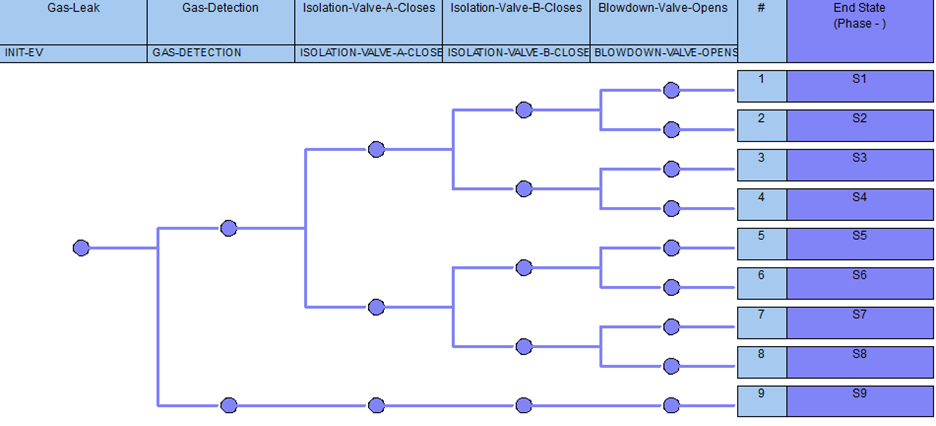
\includegraphics[width=0.9\textwidth]{3_identifying_gaps/benchmarking/datasets/figures/gas_leak_event_tree.png}
    \caption{Gas-leak event tree used in the demonstration model.}
    \label{fig:gas_leak_event_tree}
\end{figure}

Each functional event in the event tree is represented by corresponding fault trees, as shown in Figures~\ref{fig:gas_detection_fault_tree} through \ref{fig:blowdown_valve_fault_tree}.

\begin{figure}[H]
    \centering
    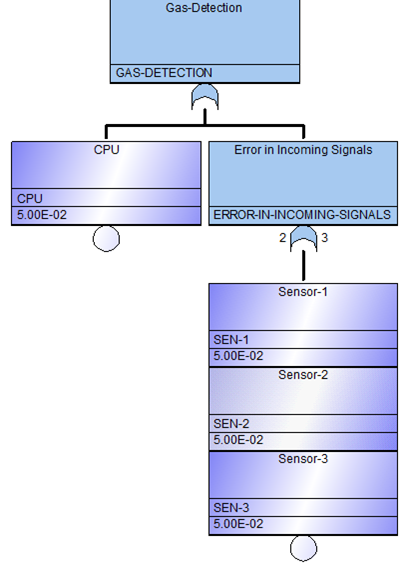
\includegraphics[width=0.4\textwidth]{3_identifying_gaps/benchmarking/datasets/figures/gas_detection_fault_tree.png}
    \caption{Gas-detection system fault tree.}
    \label{fig:gas_detection_fault_tree}
\end{figure}

\begin{figure}[H]
    \centering
    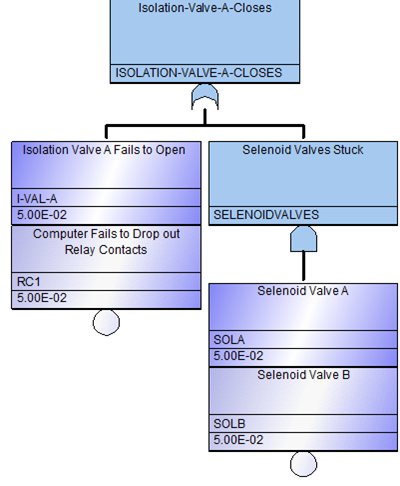
\includegraphics[width=0.4\textwidth]{3_identifying_gaps/benchmarking/datasets/figures/isolation_valve_a_fault_tree.png}
    \caption{Isolation valve A fault tree.}
    \label{fig:isolation_valve_a_fault_tree}
\end{figure}

\begin{figure}[H]
    \centering
    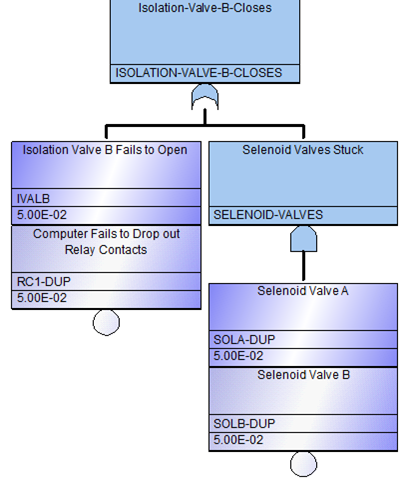
\includegraphics[width=0.4\textwidth]{3_identifying_gaps/benchmarking/datasets/figures/isolation_valve_b_fault_tree.png}
    \caption{Isolation valve B fault tree.}
    \label{fig:isolation_valve_b_fault_tree}
\end{figure}

\begin{figure}[H]
    \centering
    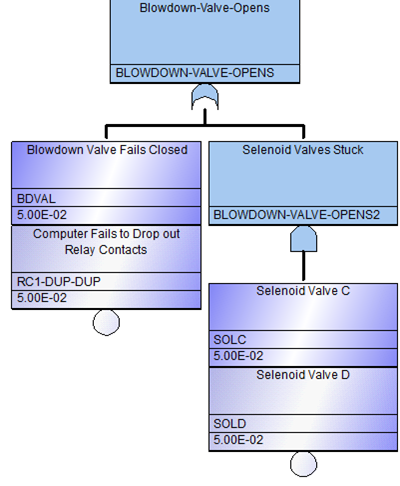
\includegraphics[width=0.4\textwidth]{3_identifying_gaps/benchmarking/datasets/figures/blowdown_valve_fault_tree.png}
    \caption{Blowdown valve fault tree.}
    \label{fig:blowdown_valve_fault_tree}
\end{figure}

The overall model exchange workflow is depicted in Figure~\ref{fig:mef_workflow}. The process is as follows: first, the model is exported from SAPHSOLVE in JSON format. Next, a Python based model converter parses the exported file, mapping its elements to internal objects. The parsed model is then converted to the OpenPSA format, with both JSON and XML representations supported. Finally, the converted model is saved in a text based format suitable for import into other PRA tools.

\begin{figure}[H]
    \centering
    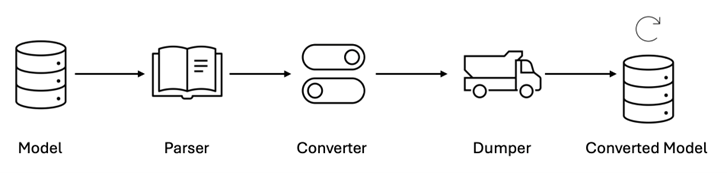
\includegraphics[width=0.7\textwidth]{3_identifying_gaps/benchmarking/datasets/figures/mef_workflow.png}
    \caption{Workflow for engine level model exchange between SAPHIRE and OpenPSA.}
    \label{fig:mef_workflow}
\end{figure}

The mapping of model elements between formats is summarized as follows: the \texttt{header} contains initiating event information, the \texttt{sysgatelist} contains functional event information, the \texttt{sequencelist} contains sequence information, the \texttt{faultreelist} contains fault tree logic, and the \texttt{eventlist} contains basic event failure data. Figure~\ref{fig:mef_demonstration} shows an overview of the mapping process.

\begin{figure}[H]
    \centering
    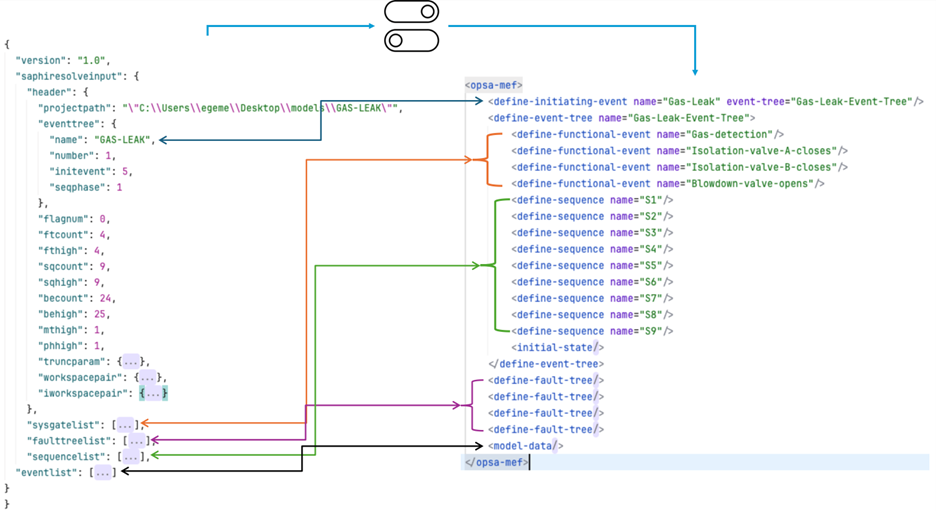
\includegraphics[width=0.9\textwidth]{3_identifying_gaps/benchmarking/datasets/figures/mef_demonstration.png}
    \caption{Demonstration of the mapping and conversion process between SAPHSOLVE and OpenPSA formats.}
    \label{fig:mef_demonstration}
\end{figure}

\subsection{Verification of Model Conversion}

To verify the correctness of the conversion, the resulting OpenPSA model is quantified using the SCRAM engine. The results are compared against those obtained from SAPHSOLVE and the original SCRAM quantification. As shown in Table~\ref{tab:mef_results_comparison}, both the number of cut sets and the computed probabilities are identical across all engines, demonstrating the fidelity of the conversion process.

\begin{table}[htbp]
    \centering
    \caption{Demo model results comparison for SCRAM and SAPHSOLVE.}
    \label{tab:mef_results_comparison}
    \begin{tabular}{|c|c|c|c|c|}
        \hline
        \textbf{Engine Sequence} & \textbf{SCRAM Probability} & \textbf{SCRAM Cut Sets} & \textbf{SAPHIRE Probability} & \textbf{SAPHIRE Cut Sets} \\
        \hline
        S1 & $1.00 \times 10^{0}$ & 1 & $1.00 \times 10^{0}$ & 1 \\
        S2 & $9.98 \times 10^{-2}$ & 3 & $9.98 \times 10^{-2}$ & 3 \\
        S3 & $9.98 \times 10^{-2}$ & 3 & $9.98 \times 10^{-2}$ & 3 \\
        S4 & $1.05 \times 10^{-2}$ & 9 & $1.05 \times 10^{-2}$ & 9 \\
        S5 & $9.98 \times 10^{-2}$ & 3 & $9.98 \times 10^{-2}$ & 3 \\
        S6 & $1.05 \times 10^{-2}$ & 9 & $1.05 \times 10^{-2}$ & 9 \\
        S7 & $1.05 \times 10^{-2}$ & 9 & $1.05 \times 10^{-2}$ & 9 \\
        S8 & $1.08 \times 10^{-3}$ & 27 & $1.08 \times 10^{-3}$ & 27 \\
        S9 & $5.71 \times 10^{-2}$ & 4 & $5.71 \times 10^{-2}$ & 4 \\
        \hline
    \end{tabular}
\end{table}